% A LaTeX template for MSc Thesis submissions to 
% Politecnico di Milano (PoliMi) - School of Industrial and Information Engineering
%
% S. Bonetti, A. Gruttadauria, G. Mescolini, A. Zingaro
% e-mail: template-tesi-ingind@polimi.it
%
% Last Revision: October 2021
%
% Copyright 2021 Politecnico di Milano, Italy. NC-BY

\documentclass{Configuration_Files/PoliMi3i_thesis}

%------------------------------------------------------------------------------
%	REQUIRED PACKAGES AND  CONFIGURATIONS
%------------------------------------------------------------------------------

% CONFIGURATIONS
\usepackage{parskip} % For paragraph layout
\usepackage{setspace} % For using single or double spacing
\usepackage{emptypage} % To insert empty pages
\usepackage{multicol} % To write in multiple columns (executive summary)
\setlength\columnsep{15pt} % Column separation in executive summary
\setlength\parindent{0pt} % Indentation
\raggedbottom  

% PACKAGES FOR TITLES
\usepackage{titlesec}
% \titlespacing{\section}{left spacing}{before spacing}{after spacing}
\titlespacing{\section}{0pt}{3.3ex}{2ex}
\titlespacing{\subsection}{0pt}{3.3ex}{1.65ex}
\titlespacing{\subsubsection}{0pt}{3.3ex}{1ex}
\usepackage{color}

% PACKAGES FOR LANGUAGE AND FONT
\usepackage[english]{babel} % The document is in English  
\usepackage[utf8]{inputenc} % UTF8 encoding
\usepackage[T1]{fontenc} % Font encoding
\usepackage[11pt]{moresize} % Big fonts

% PACKAGES FOR IMAGES
\usepackage{graphicx}
\usepackage{transparent} % Enables transparent images
\usepackage{eso-pic} % For the background picture on the title page
\usepackage{subfig} % Numbered and caption subfigures using \subfloat.
\usepackage{tikz} % A package for high-quality hand-made figures.
\usetikzlibrary{}
\graphicspath{{./Images/}} % Directory of the images
\usepackage{caption} % Coloured captions
\usepackage{xcolor} % Coloured captions
\usepackage{amsthm,thmtools,xcolor} % Coloured "Theorem"
\usepackage{float}

% STANDARD MATH PACKAGES
\usepackage{amsmath}
\usepackage{amsthm}
\usepackage{amssymb}
\usepackage{amsfonts}
\usepackage{bm}
\usepackage[overload]{empheq} % For braced-style systems of equations.
\usepackage{fix-cm} % To override original LaTeX restrictions on sizes

% PACKAGES FOR TABLES
\usepackage{tabularx}
\usepackage{longtable} % Tables that can span several pages
\usepackage{colortbl}

% PACKAGES FOR ALGORITHMS (PSEUDO-CODE)
\usepackage{algorithm}
\usepackage{algorithmic}

% PACKAGES FOR REFERENCES & BIBLIOGRAPHY
\usepackage[colorlinks=true,linkcolor=black,anchorcolor=black,citecolor=black,filecolor=black,menucolor=black,runcolor=black,urlcolor=black]{hyperref} % Adds clickable links at references
\usepackage{cleveref}
\usepackage[square, numbers, sort&compress]{natbib} % Square brackets, citing references with numbers, citations sorted by appearance in the text and compressed
\bibliographystyle{abbrvnat} % You may use a different style adapted to your field

% OTHER PACKAGES
\usepackage{pdfpages} % To include a pdf file
\usepackage{afterpage}
\usepackage{lipsum} % DUMMY PACKAGE
\usepackage{fancyhdr} % For the headers
\fancyhf{}

% Input of configuration file. Do not change config.tex file unless you really know what you are doing. 
% Define blue color typical of polimi
\definecolor{bluepoli}{cmyk}{0.4,0.1,0,0.4}

% Custom theorem environments
\declaretheoremstyle[
  headfont=\color{bluepoli}\normalfont\bfseries,
  bodyfont=\color{black}\normalfont\itshape,
]{colored}

% Set-up caption colors
\captionsetup[figure]{labelfont={color=bluepoli}} % Set colour of the captions
\captionsetup[table]{labelfont={color=bluepoli}} % Set colour of the captions
\captionsetup[algorithm]{labelfont={color=bluepoli}} % Set colour of the captions

\theoremstyle{colored}
\newtheorem{theorem}{Theorem}[chapter]
\newtheorem{proposition}{Proposition}[chapter]

% Enhances the features of the standard "table" and "tabular" environments.
\newcommand\T{\rule{0pt}{2.6ex}}
\newcommand\B{\rule[-1.2ex]{0pt}{0pt}}

% Pseudo-code algorithm descriptions.
\newcounter{algsubstate}
\renewcommand{\thealgsubstate}{\alph{algsubstate}}
\newenvironment{algsubstates}
  {\setcounter{algsubstate}{0}%
   \renewcommand{\STATE}{%
     \stepcounter{algsubstate}%
     \Statex {\small\thealgsubstate:}\space}}
  {}

% New font size
\newcommand\numfontsize{\@setfontsize\Huge{200}{60}}

% Title format: chapter
\titleformat{\chapter}[hang]{
\fontsize{50}{20}\selectfont\bfseries\filright}{\textcolor{bluepoli} \thechapter\hsp\hspace{2mm}\textcolor{bluepoli}{|   }\hsp}{0pt}{\huge\bfseries \textcolor{bluepoli}
}

% Title format: section
\titleformat{\section}
{\color{bluepoli}\normalfont\Large\bfseries}
{\color{bluepoli}\thesection.}{1em}{}

% Title format: subsection
\titleformat{\subsection}
{\color{bluepoli}\normalfont\large\bfseries}
{\color{bluepoli}\thesubsection.}{1em}{}

% Title format: subsubsection
\titleformat{\subsubsection}
{\color{bluepoli}\normalfont\large\bfseries}
{\color{bluepoli}\thesubsubsection.}{1em}{}

% Shortening for setting no horizontal-spacing
\newcommand{\hsp}{\hspace{0pt}}

\makeatletter
% Renewcommand: cleardoublepage including the background pic
\renewcommand*\cleardoublepage{%
  \clearpage\if@twoside\ifodd\c@page\else
  \null
  \AddToShipoutPicture*{\BackgroundPic}
  \thispagestyle{empty}%
  \newpage
  \if@twocolumn\hbox{}\newpage\fi\fi\fi}
\makeatother

%For correctly numbering algorithms
\numberwithin{algorithm}{chapter}

%----------------------------------------------------------------------------
%	BEGIN OF YOUR DOCUMENT
%----------------------------------------------------------------------------

\begin{document}

\fancypagestyle{plain}{
\fancyhf{} % Clear all header and footer fields
\fancyhead[RO,RE]{\thepage} %RO=right odd, RE=right even
\renewcommand{\headrulewidth}{0pt}
\renewcommand{\footrulewidth}{0pt}}

%----------------------------------------------------------------------------
%	TITLE PAGE
%----------------------------------------------------------------------------

\pagestyle{empty} % No page numbers
\frontmatter % Use roman page numbering style (i, ii, iii, iv...) for the preamble pages

\puttitle{
	title=US GDP \& Inflation, % Title
    course=Bayesian Learning and Montecarlo Simulation, % Course
	academicyear={2023-24},  % Academic Year
} % These info will be put into your Title page 

\startpreamble
\setcounter{page}{1} % Set page counter to 1

%----------------------------------------------------------------------------
%	LIST OF CONTENTS/FIGURES/TABLES/SYMBOLS
%----------------------------------------------------------------------------

% TABLE OF CONTENTS
\tableofcontents % Table of contents 

%-------------------------------------------------------------------------
%	THESIS MAIN TEXT
%-------------------------------------------------------------------------
% In the main text of your thesis you can write the chapters in two different ways:
%
%(1) As presented in this template you can write:
%    \chapter{Title of the chapter}
%    *body of the chapter*
%
%(2) You can write your chapter in a separated .tex file and then include it in the main file with the following command:
%    \chapter{Title of the chapter}
%    \input{chapter_file.tex}
%
% Especially for long thesis, we recommend you the second option.

\addtocontents{toc}{\vspace{2em}} % Add a gap in the Contents, for aesthetics
\mainmatter % Begin numeric (1,2,3...) page numbering

% --------------------------------------------------------------------------
%    NUMBERED CHAPTERS 
% --------------------------------------------------------------------------
\chapter{Problem Description}
\chapter{Autoregressive Model}
\label{AR}
The Autoregressive Model(AR) is a model for time series analysis. The model specifies that the output variable depends 
linearly on its own previous values and on a stochastic term. An autoregression model of order p can be written as:
\begin{equation}
    y_{t}=\mu_{0}+\epsilon_t \sum^{p}_{i=1}\alpha_{i} y_{t-i}
\end{equation}
where $\mu_{0}$ is the mean of the timeserie, $\alpha_{i}$ are the parameters of the model, $\epsilon_{t}$ is white noise and $y_{t-1}, y_{t-2}, ..., y_{t-p}$ are the past values.

We decided to implement the $p=1$ AR model, which can be rewritten in the following way:
\begin{equation}
    \label{AR_q1}
    y_{t}=\mu_{0}+\epsilon_t +\alpha y_{t-1} \qquad 
    \epsilon_t \stackrel{iid}{\sim} \mathcal{N}(0,\sigma^2)
\end{equation}
and we assumed $\epsilon$ to be independent and identical distributed variables coming from a normal distribution with mean $0$ and variance $\sigma^2$.

Note that the stationarity of the model is garanteed for $|\alpha|<1$.

\section*{AR(1)}
Given the equation \refeq{AR_q1} the likelihood of the AR model can be expressed as:
\begin{equation}
    y_{t}|\mu_{0},\alpha,\sigma^2,y_{t-1}\sim \mathcal{N}(\mu_{0} + \alpha y_{t-1}, \sigma^2)
\end{equation}
We chose the following priors:
\begin{equation}
    \begin{split}
        \mu_0 \sim \mathcal{N}(0.0, 10000) \\
        \tau = 1 / \sigma^2 \sim \mathcal{G}(2, 0.1) \\
        \alpha \sim \mathcal{U}(-1.0, 1.0)
    \end{split}
\end{equation}
Since we lack prior information for this problem, we selected hyperparameters for $\mu_{0}$ and $\sigma^2$ to ensure uninformative distributions, while for $\alpha$ we chose a uniform distribution between -1 and 1 in order to respect the stationary constraint mentioned before.
We analyzed trace plots and autocorrelation plots to verify the model's correctness and the validity of our assumptions.
Now, by running the JAGS code that implements the MA model of order 1 for the GDP and for the inflation, we obtain the following posteriors: \\
\begin{figure}[h]
    \centering
    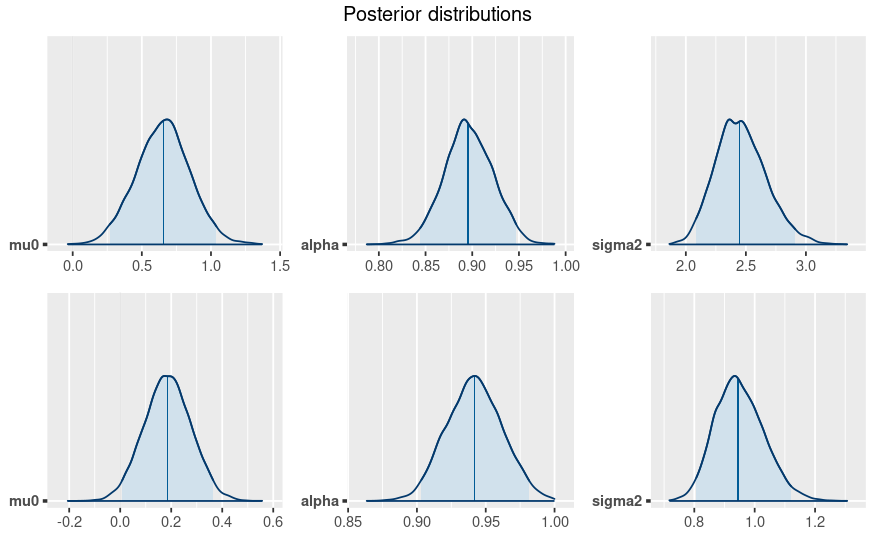
\includegraphics[width=\textwidth]{../Images/2-AR/posteriors.png}
    \caption{The image displays the posterior distributions of the parameters for the AR(1) model. The top line corresponds to the model used for GDP, while the bottom line corresponds to the model used for inflation.}
    \label{fig:AR_posteriors}
\end{figure} \\
Once we assested the validity of the results, we plotted the in-sample and out-of-sample prediction with credible intervals and we compared it with the true data: \\
\begin{figure}[H]
    \centering
    \begin{minipage}[H]{0.7\textwidth}
        \centering
        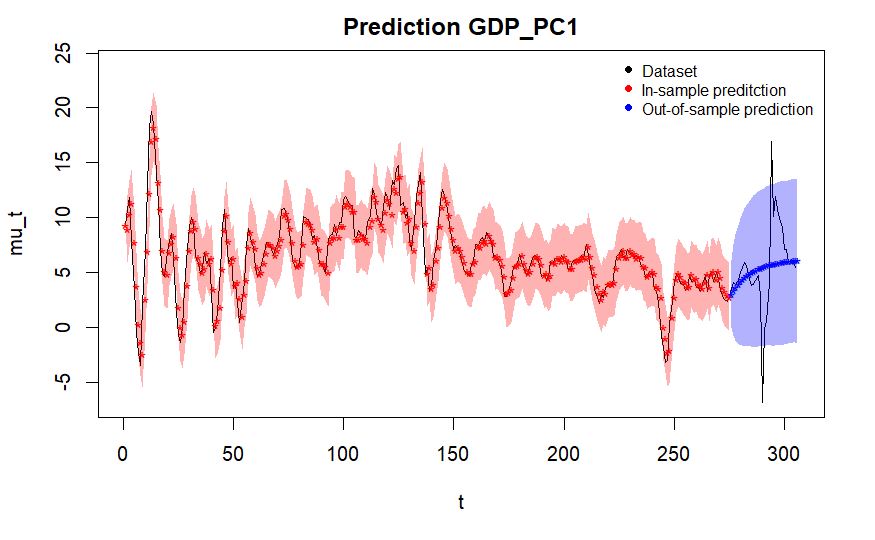
\includegraphics[width=\textwidth]{../Images/2-AR/gdp_prediction.png}
        \label{fig:first}
    \end{minipage}
    \begin{minipage}[H]{0.7\textwidth}
        \centering
        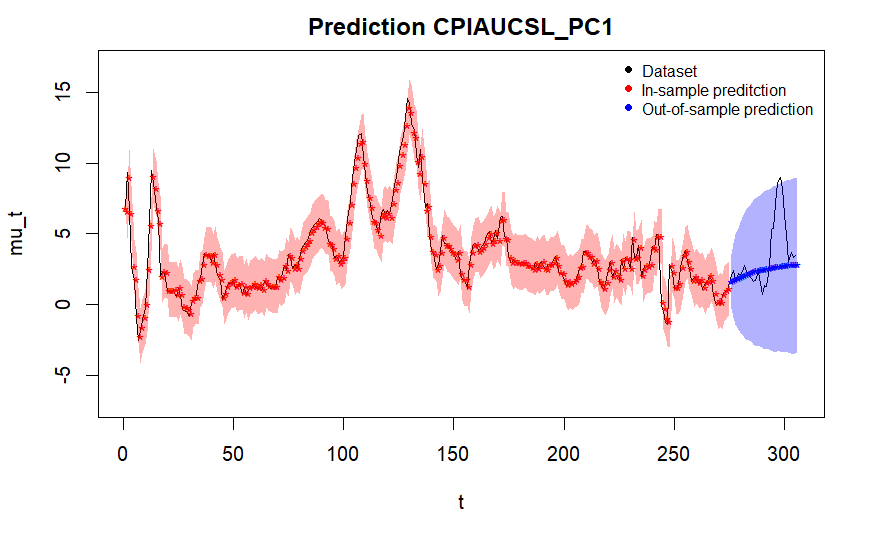
\includegraphics[width=\textwidth]{../Images/2-AR/infl_prediction.png}
        \label{fig:second}
    \end{minipage}
    \caption{In-sample and out-of-sample predictions}
    \label{fig:combined}
\end{figure} \\

We concluded by comparing the model's in-sample predictions and the posterior distributions of its parameters with those obtained from the AR model using the ARIMA function. The detailed comparison results are provided in the Appendix. It was found that there is no significant difference between them. 
\section{Moving Average Model}
\label{sec:MA}
A Moving Average (MA) model is another approach used in univariate time series analysis. Unlike the Autoregressive (AR) model, where the target variable depends on its past values, the MA model relies on past errors. \\
Formally, a Moving Average model of order $q$ is represented as:
\begin{equation}
    \label{eq:MA}
    y_{t} = \mu_{0} + \sum^{q}_{i=1} \theta_{i} \epsilon_{t-i} + \epsilon_t
\end{equation}
where $q$ is the number of past errors considered, $\mu_{0}$ is the mean of the series, $\theta_{1}, \theta_{2}, ..., \theta_{q}$ are the model coefficients, and $\epsilon_{t}, \epsilon_{t-1}, ..., \epsilon_{t-q}$ are the error terms. \\
For our analysis, we first implemented the MA model of order 1 (MA(1)). Then, by examining the autocorrelation plots for the two time series, we noticed a significant correlation at 2 lags. Consequently, we concluded that an MA model of order 2 (MA(2)) would perform better, and we implemented it.
\subsection*{MA(1)}
The MA(1) model is defined as follows:
\begin{equation}
    \label{eq:MA1}
    y_{t} = \mu_{0} + \theta \epsilon_{t-1} + \epsilon_t
\end{equation}
In our case study, we assume that $\epsilon_t$ are independent and identically distributed variables from a normal distribution with mean $0$ and variance $\sigma^2$, i.e., $\epsilon_t \stackrel{iid}{\sim} \mathcal{N}(0,\sigma^2)$, leading to the following likelihood:
\begin{equation}
    \label{eq:MA1_likelihood}
    y_{t}|\mu_{0},\theta,\sigma^2,\epsilon_{t-1} \sim \mathcal{N}(\mu_{0} + \theta \epsilon_{t-1}, \sigma^2)
\end{equation}
For the priors, we chose:
\begin{equation}
    \label{eq:MA1_priors}
    \begin{split}
        \mu_0 \sim \mathcal{N}(0.0, 10000) \\
        \tau = 1 / \sigma^2 \sim \mathcal{G}(2, 0.1) \\
        \theta \sim \mathcal{U}(-1.0, 1.0)
    \end{split}
\end{equation}
We selected uninformative priors for all the parameters: $\mu_{0}$, $\sigma^2$, and $\theta$. \\
Running the JAGS code to implement the MA(1) model for GDP and CPIAUCSL, we obtained the posterior distributions shown in Figure \ref{fig:MA1_posteriors}, with the corresponding means and 95\% credible intervals reported in Table \ref{tab:MA1_posteriors}. \\
\begin{figure}[h]
    \centering
    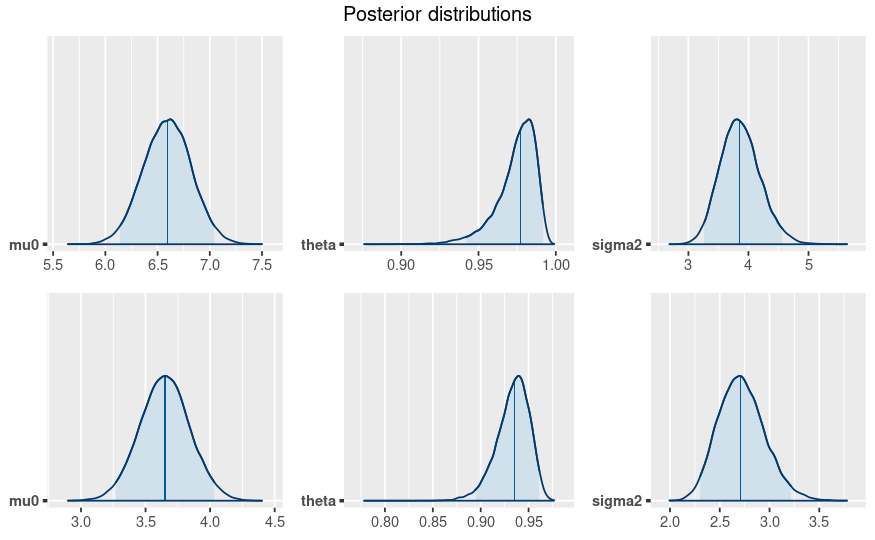
\includegraphics[width=0.8\textwidth]{images/3-MA/posteriors.png}
    \caption{Posterior distributions of the parameters for the MA(1) models. The top line corresponds to the model used for GDP, while the bottom line corresponds to the model used for CPIAUCSL.}
    \label{fig:MA1_posteriors}
\end{figure}
\begin{table}[H]
    \centering
    \begin{tabular}{|c|c|c|c|}
        \hline
        \textbf{Model target variable } & \textbf{Parameter } & \textbf{Posterior Mean } & \textbf{95\% Credible Interval } \\
        \hline
        GDP      & $\mu_0$    & 6.5934423 & (6.1441382, 7.0421211) \\
        GDP      & $\theta$   & 0.9745347 & (0.9419309, 0.9915436) \\
        GDP      & $\sigma^2$ & 3.8669139 & (3.2666059, 4.5663869) \\
        CPIAUCSL & $\mu_0$    & 3.6496595 & (3.2718468, 4.0311333) \\
        CPIAUCSL & $\theta$   & 0.9335022 & (0.8946139, 0.9613808) \\
        CPIAUCSL & $\sigma^2$ & 2.7205353 & (2.3038087, 3.2125894) \\
        \hline
    \end{tabular}
    \caption{Posterior means and 95\% credible intervals for the parameters of the MA(1) models.}
    \label{tab:MA1_posteriors}
\end{table}
In both the GDP and CPIAUCSL models, the $\theta$ parameter is close to 1. However, using a prior for $\theta$ over a larger range, i.e., $\theta \sim \mathcal{U}(-2.0, 2.0)$, did not significantly change the estimated value of $\theta$. \\
We also examined the trace plots and autocorrelation plots and found no significant issues. \\
Finally, plotting the in-sample and out-of-sample predictions with 95\% credible intervals and comparing them with the actual data, we obtained the results shown in Figures \ref{fig:MA1_gdp_prediction} and \ref{fig:MA1_infl_prediction}. As observed, the MA(1) model is not good for out of sample predictions, as it fails to capture the trend of the data and returns a flat line.
\begin{figure}[H]
    \centering
    \begin{minipage}{0.49\textwidth}
        \centering
        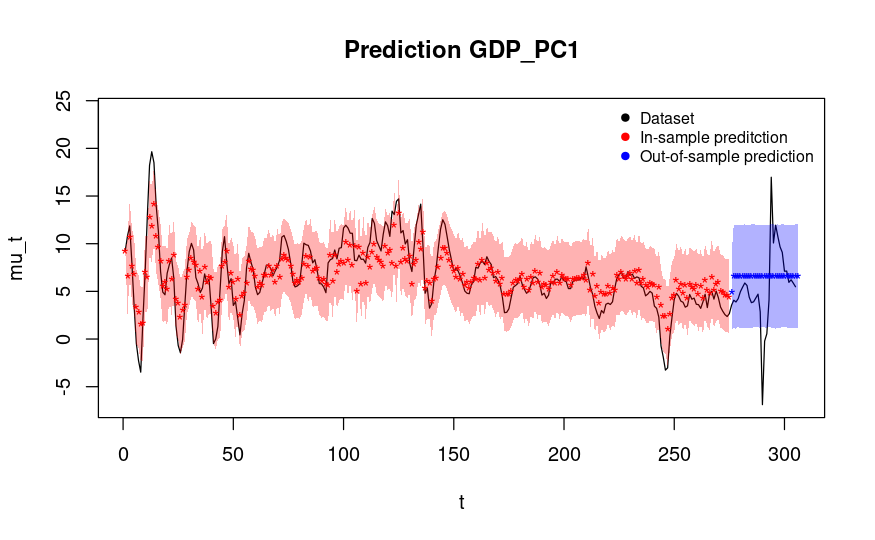
\includegraphics[width=\textwidth]{images/3-MA/gdp_prediction.png}
        \caption{In-sample and out-of-sample predictions for the GDP using the MA(1) model.}
        \label{fig:MA1_gdp_prediction}
    \end{minipage}\hfill
    \begin{minipage}{0.49\textwidth}
        \centering
        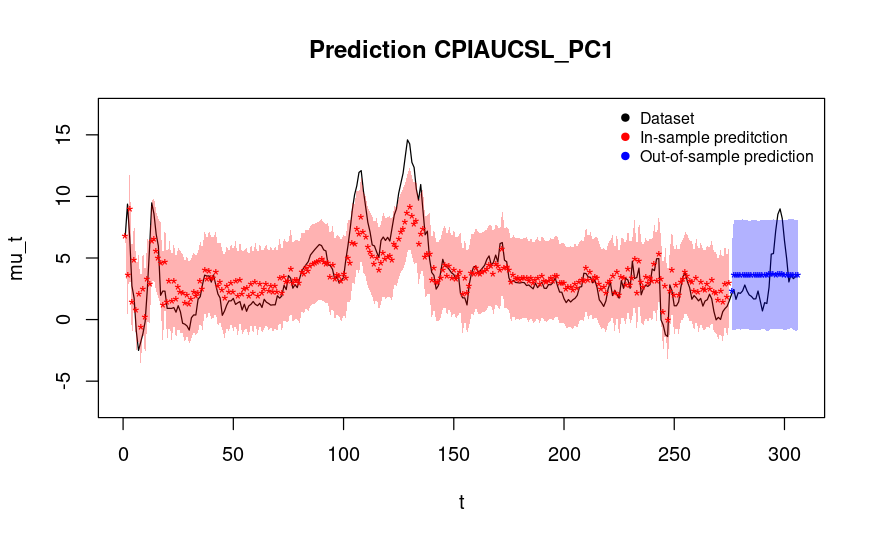
\includegraphics[width=\textwidth]{images/3-MA/infl_prediction.png}
        \caption{In-sample and out-of-sample predictions for the CPIAUCSL using the MA(1) model.}
        \label{fig:MA1_infl_prediction}
    \end{minipage}
\end{figure}
We also compared the model's in-sample predictions and posterior distributions with those obtained from the MA model using the ARIMA function. Detailed comparison results are provided in the Appendix, showing no significant differences between them.
\subsection*{MA(2)}
The MA(2) model is defined as follows:
\begin{equation}
    \label{eq:MA2}
    y_{t} = \mu_{0} + \theta_1 \epsilon_{t-1} + \theta_2 \epsilon_{t-2} + \epsilon_t
\end{equation}
In our case study, we assume that $\epsilon_t$ are independent and identically distributed variables from a normal distribution with mean $0$ and variance $\sigma^2$, i.e., $\epsilon_t \stackrel{iid}{\sim} \mathcal{N}(0,\sigma^2)$, leading to the following likelihood:
\begin{equation}
    \label{eq:MA2_likelihood}
    y_{t}|\mu_{0},\theta_1,\theta_2,\sigma^2,\epsilon_{t-1},\epsilon_{t-2} \sim \mathcal{N}(\mu_{0} + \theta_1 \epsilon_{t-1} + \theta_2 \epsilon_{t-2}, \sigma^2)
\end{equation}
For the priors, we chose:
\begin{equation}
    \label{eq:MA2_priors}
    \begin{split}
        \mu_0 \sim \mathcal{N}(0.0, 10000) \\
        \tau = 1 / \sigma^2 \sim \mathcal{G}(2, 0.1) \\
        \theta_1 \sim \mathcal{U}(-1.5, 1.5) \\
        \theta_2 \sim \mathcal{U}(-1.0, 1.0)
    \end{split}
\end{equation}
We selected uninformative priors for $\mu_{0}$, $\sigma^2$, $\theta_1$, and $\theta_2$. \\
Running the JAGS code to implement the MA(2) model for GDP and CPIAUCSL, we obtained the posterior distributions shown in Figure \ref{fig:MA2_posteriors}, with the corresponding means and 95\% credible intervals reported in Table \ref{tab:MA2_posteriors}. \\
\begin{figure}[H]
    \centering
    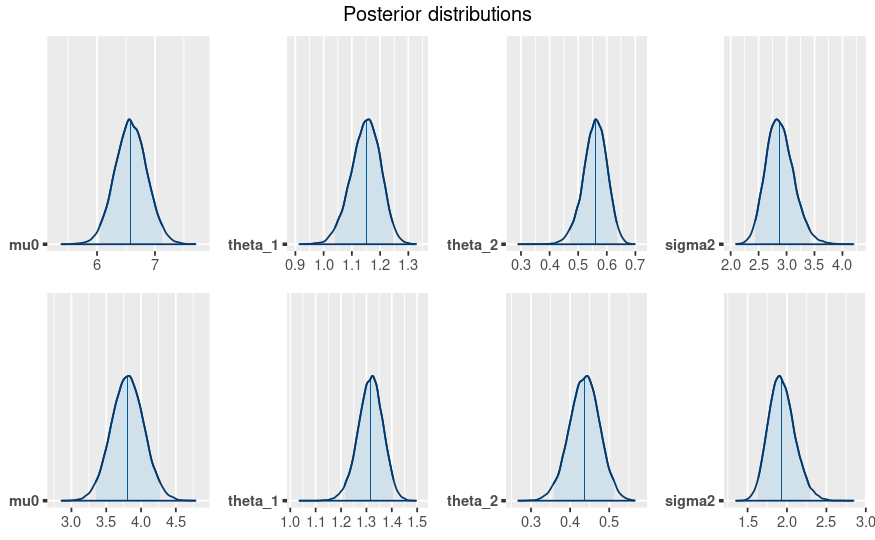
\includegraphics[width=0.8\textwidth]{images/3-MA/posteriors2.png}
    \caption{Posterior distributions of the parameters for the MA(2) models. The top line corresponds to the model used for GDP, while the bottom line corresponds to the model used for CPIAUCSL.}
    \label{fig:MA2_posteriors}
\end{figure} 
\begin{table}[H]
    \centering
    \begin{tabular}{|c|c|c|c|}
        \hline
        \textbf{Model target variable } & \textbf{Parameter } & \textbf{Posterior Mean } & \textbf{95\% Credible Interval } \\
        \hline
        GDP      & $\mu_0$    & 6.5862752 & (6.0523533, 7.1291252) \\
        GDP      & $\theta_1$ & 1.1489023 & (1.0408063, 1.2447200) \\
        GDP      & $\theta_2$ & 0.5587509 & (0.4698359, 0.6348533) \\
        GDP      & $\sigma^2$ & 2.8842617 & (2.4383601, 3.4118375) \\
        CPIAUCSL & $\mu_0$    & 3.8081535 & (3.3497252, 4.2727049) \\
        CPIAUCSL & $\theta_1$ & 1.3155230 & (1.2142974, 1.4063565) \\
        CPIAUCSL & $\theta_2$ & 0.4365283 & (0.3581476, 0.5111502) \\
        CPIAUCSL & $\sigma^2$ & 1.9356539 & (1.6371395, 2.2893457) \\
        \hline
    \end{tabular}
    \caption{Posterior means and 95\% credible intervals for the parameters of the MA(2) models.}
    \label{tab:MA2_posteriors}
\end{table}
Plotting the in-sample and out-of-sample predictions with 95\% credible intervals and comparing them with the actual data, we obtained the results shown in Figures \ref{fig:MA2_gdp_prediction} and \ref{fig:MA2_infl_prediction}. \\
As with the MA(1) model, the MA(2) model is not good for out-of-sample predictions, as it fails to capture the trend of the data and returns a flat line.
\begin{figure}[H]
    \centering
    \begin{minipage}{0.49\textwidth}
        \centering
        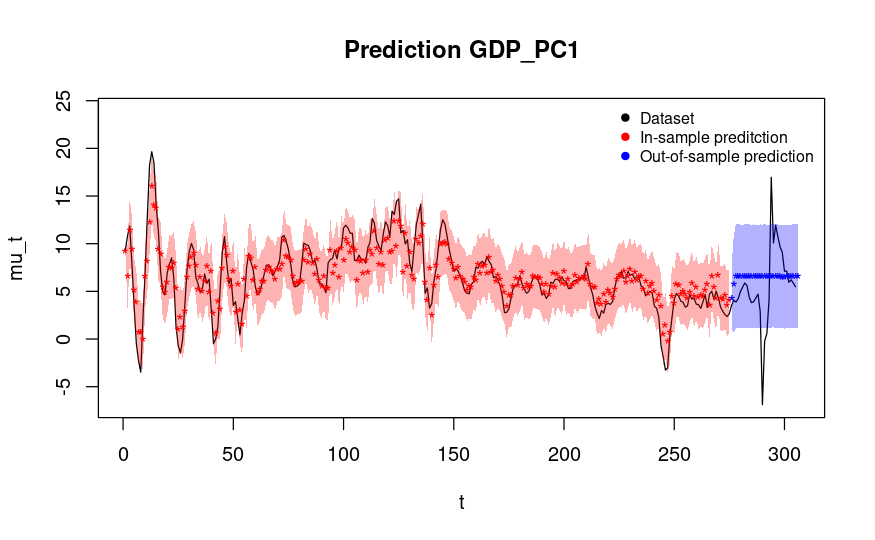
\includegraphics[width=\textwidth]{images/3-MA/gdp_prediction2.png}
        \caption{In-sample and out-of-sample predictions for the GDP using the MA(2) model.}
        \label{fig:MA2_gdp_prediction}
    \end{minipage}\hfill
    \begin{minipage}{0.49\textwidth}
        \centering
        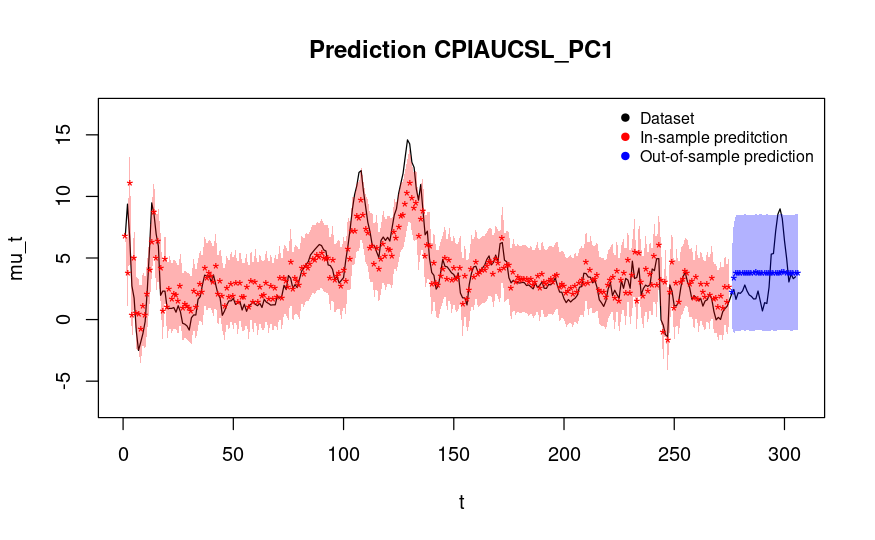
\includegraphics[width=\textwidth]{images/3-MA/infl_prediction2.png}
        \caption{In-sample and out-of-sample predictions for the CPIAUCSL using the MA(2) model.}
        \label{fig:MA2_infl_prediction}
    \end{minipage}
\end{figure}
In the end, we compared the model's in-sample predictions and posterior distributions with those obtained from the MA model using the ARIMA function. Detailed comparison results are provided in the Appendix, showing no significant differences between them.
\section{Autoregressive Moving Average Model}
\label{sec:ARMA}
The Autoregressive Moving Average Model (ARMA) is obtained by merging the AR and MA models. \\
Formally, the ARMA model of order $(p, q)$ is represented as follows:
\begin{equation}
    \label{eq:ARMA}
    y_{t} = \mu_{0} + \sum^{p}_{i=1}\alpha_{i} y_{t-i} + \sum^{q}_{j=1}\theta_{j} \epsilon_{t-j} + \epsilon_t 
\end{equation}
where $p$ is the number of past values considered in the AR part, $q$ is the number of past errors considered in the MA part, $\mu_{0}$ is a constant, $\alpha_{i}$ and $\theta_{j}$ are the model parameters, $y_{t-1}, y_{t-2}, ..., y_{t-p}$ are the past values, and $\epsilon_{t}, \epsilon_{t-1}, ..., \epsilon_{t-q}$ are the error terms. \\
For our analysis, we decided to implement only the ARMA(1,1) model.
\subsection*{ARMA(1,1)}
The ARMA(1,1) model is defined as:
\begin{equation}
    \label{eq:ARMA1,1}
    y_{t} = \mu_{0} + \alpha y_{t-1} + \theta \epsilon_{t-1} + \epsilon_t
\end{equation}
In our case study, we assume that $\epsilon_t$ are independent and identically distributed variables from a normal distribution with mean $0$ and variance $\sigma^2$, i.e., $\epsilon_t \stackrel{iid}{\sim} \mathcal{N}(0,\sigma^2)$, leading to the following likelihood:
\begin{equation}
    \label{eq:ARMA1,1_likelihood}
    y_{t}|\mu_{0},\alpha,\theta,\sigma^2,y_{t-1},\epsilon_{t-1} \sim \mathcal{N}(\mu_{0} + \alpha y_{t-1} + \theta \epsilon_{t-1}, \sigma^2)
\end{equation}
For the priors, we chose:
\begin{equation}
    \label{eq:ARMA1,1_priors}
    \begin{split}
        \mu_0 \sim \mathcal{N}(0.0, 10000) \\
        \tau = 1 / \sigma^2 \sim \mathcal{G}(2, 0.1) \\
        \alpha \sim \mathcal{U}(-1.0, 1.0) \\
        \theta \sim \mathcal{U}(-1.0, 1.0)
    \end{split}
\end{equation}
We selected uninformative priors for all the parameters: $\mu_{0}$, $\sigma^2$, $\alpha$, and $\theta$. \\
Running the JAGS code to implement the ARMA(1,1) model for GDP and CPIAUCSL, we obtained the posterior distributions shown in Figure \ref{fig:ARMA1,1_posteriors}, with the corresponding means and 95\% credible intervals reported in Table \ref{tab:ARMA1,1_posteriors}.
\begin{figure}[H]
    \centering
    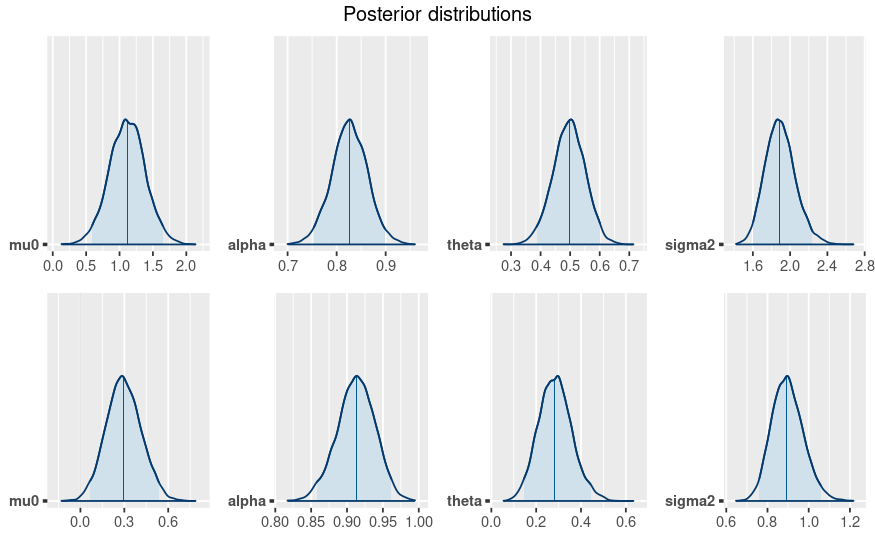
\includegraphics[width=0.8\textwidth]{images/4-ARMA/posteriors.png}
    \caption{Posterior distributions of the parameters for the ARMA(1,1) models. The top line corresponds to the model used for GDP, while the bottom line corresponds to the model used for CPIAUCSL.}
    \label{fig:ARMA1,1_posteriors}
\end{figure}
\begin{table}[H]
    \centering
    \begin{tabular}{|c|c|c|c|}
        \hline
        \textbf{Model target variable } & \textbf{Parameter } & \textbf{Posterior Mean } & \textbf{95\% Credible Interval } \\
        \hline
        GDP      & $\mu_0$    & 1.1207710 & (0.59421700, 1.6538357) \\
        GDP      & $\alpha$   & 0.8254802 & (0.75268077, 0.8966752) \\
        GDP      & $\theta$   & 0.4952213 & (0.38504175, 0.6024967) \\
        GDP      & $\sigma^2$ & 1.8977382 & (1.60426034, 2.2438487) \\
        CPIAUCSL & $\mu_0$    & 0.2941814 & (0.07023124, 0.5314746) \\
        CPIAUCSL & $\alpha$   & 0.9127231 & (0.86025773, 0.9612327) \\
        CPIAUCSL & $\theta$   & 0.2846962 & (0.14830563, 0.4392942) \\
        CPIAUCSL & $\sigma^2$ & 0.8976673 & (0.75858882, 1.0607612) \\
        \hline
    \end{tabular}
    \caption{Posterior means and 95\% credible intervals for the parameters of the ARMA(1,1) models.}
    \label{tab:ARMA1,1_posteriors}
\end{table}
Plotting the in-sample and out-of-sample predictions with 95\% credible intervals and comparing them with the actual data, we obtained the results shown in Figures \ref{fig:ARMA1,1_gdp_prediction} and \ref{fig:ARMA1,1_infl_prediction}. \\
The out-of-sample predictions for GDP and CPIAUCSL effectively capture the initial data trends. Nevertheless, the ARMA(1,1) model fails to anticipate the significant impact of the COVID-19 pandemic, which is completely understandable.
\begin{figure}[H]
    \centering
    \begin{minipage}{0.5\textwidth}
        \centering
        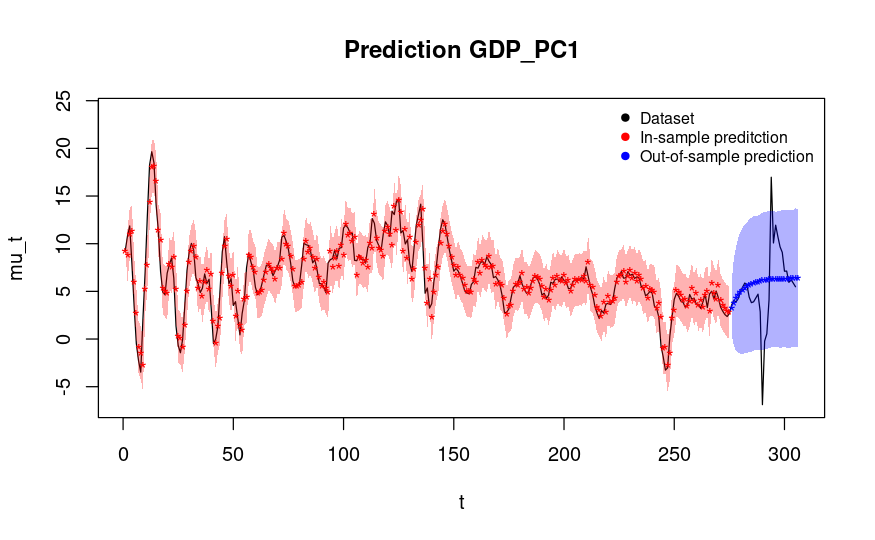
\includegraphics[width=\textwidth]{images/4-ARMA/gdp_prediction.png}
        \caption{In-sample and out-of-sample predictions for the GDP using the ARMA(1,1) model.}
        \label{fig:ARMA1,1_gdp_prediction}
    \end{minipage}\hfill
    \begin{minipage}{0.5\textwidth}
        \centering
        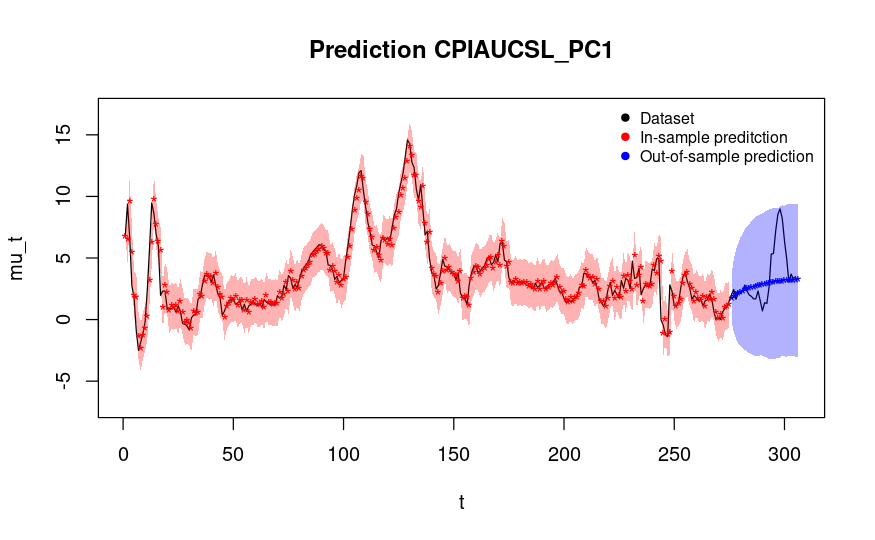
\includegraphics[width=\textwidth]{images/4-ARMA/infl_prediction.png}
        \caption{In-sample and out-of-sample predictions for the CPIAUCSL using the ARMA(1,1) model.}
        \label{fig:ARMA1,1_infl_prediction}
    \end{minipage}
\end{figure}
Finally, examining the trace plots and autocorrelation plots, we found no significant issues, and comparing our model with the one obtained using the ARIMA function, we observed that the two models have similar results. Results are provided in the Appendix.
\chapter{GARCH}
\chapter{VAR}
\label{VAR}

\begin{figure}[h]
    \centering
    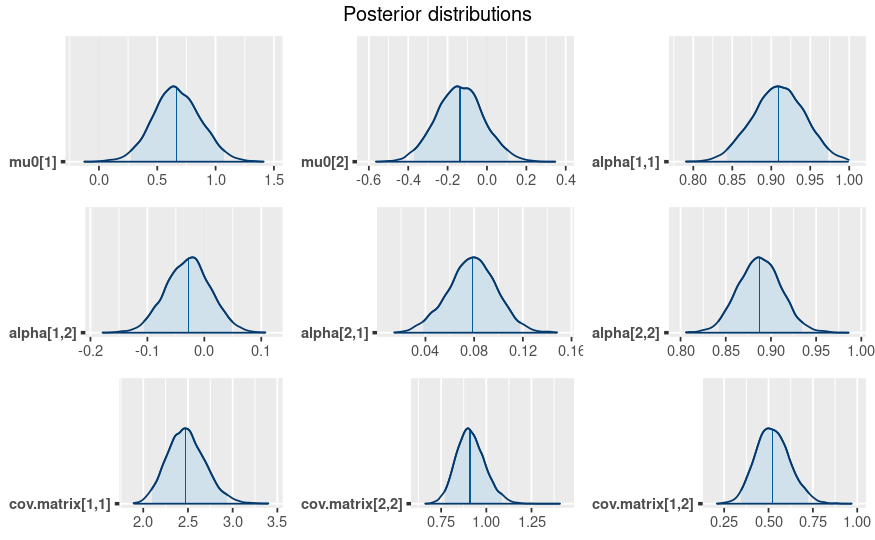
\includegraphics[width=\textwidth]{../Images/6-VAR/posteriors.png}
    \caption{The image displays the posterior distributions of the parameters for the VAR(1) model.}
    \label{fig:VAR_posteriors}
\end{figure}

\begin{figure}[h]
    \centering
    \begin{minipage}[t]{0.7\textwidth}
        \centering
        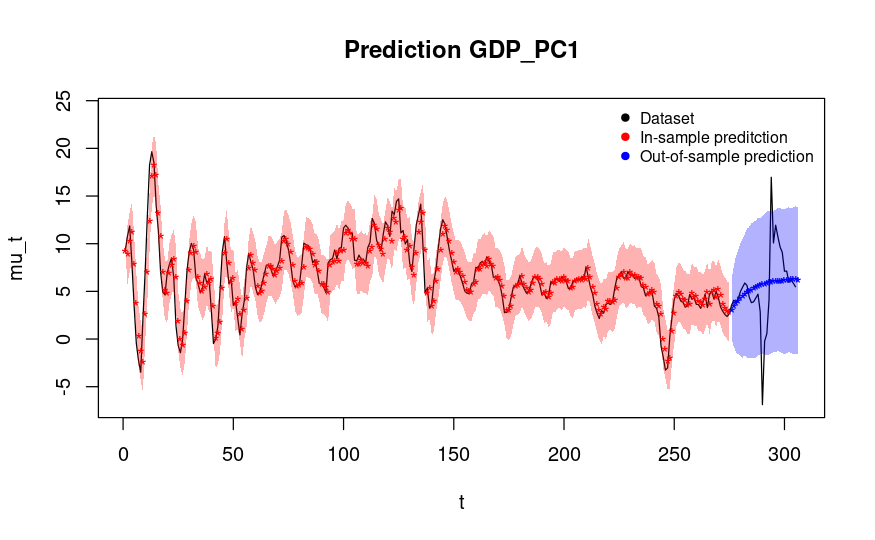
\includegraphics[width=\textwidth]{../Images/6-VAR/gdp_prediction.png}
        \label{fig:VAR_first}
    \end{minipage}
    \begin{minipage}[t]{0.7\textwidth}
        \centering
        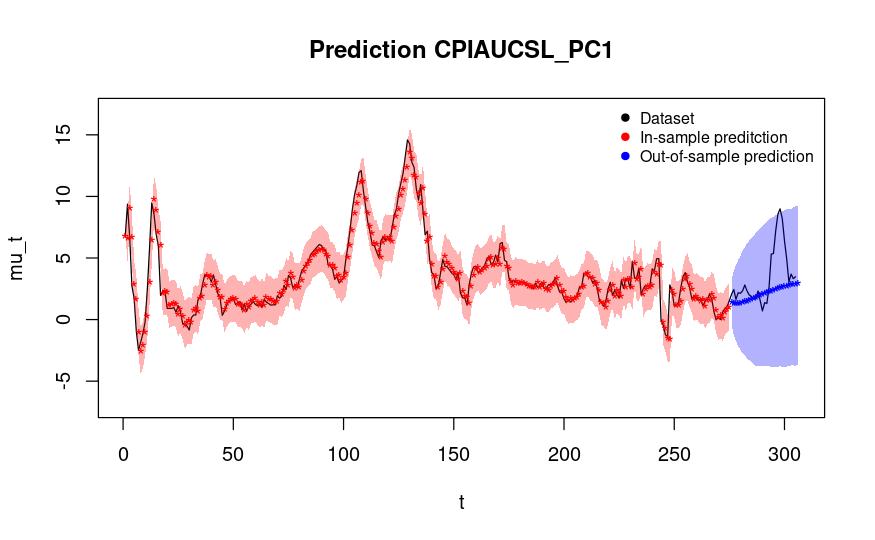
\includegraphics[width=\textwidth]{../Images/6-VAR/infl_prediction.png}
        \label{fig:VAR_second}
    \end{minipage}
    \caption{VAR(1): In-sample and out-of-sample predictions}
    \label{fig:VAR_combined}
\end{figure}

\end{document}
